\documentclass[xcolor={usenames,dvipsnames,svgnames}, compress, aspectratio=169, 11pt]{beamer}

\usepackage{booktabs}
\usepackage{multirow}
\usepackage{dcolumn}
\usepackage{colortbl}
\usepackage{xcolor}
\usepackage{hyperref}
\usepackage{amsmath}
\usepackage{wrapfig}
\usepackage{algorithm}
\usepackage[noend]{algpseudocode} 
\usepackage{pifont}
\usepackage[style=authoryear-icomp,backend=bibtex, mincitenames=2, maxcitenames=2]{biblatex}
\usepackage{marvosym}
\usepackage{mathtools}
\usepackage{array}
\usepackage[export]{adjustbox}
\usepackage{bm}
\usepackage{dsfont}
\usepackage{subcaption}

\usepackage[font=scriptsize]{caption}

\newcommand{\argmax}{\operatornamewithlimits{argmax}}
\newcommand{\argmin}{\operatornamewithlimits{argmin}}
\newcommand{\nodeset}[1]{\bm{\mathsf{#1}}}
\newcommand{\cbar}{\,|\,}
\newcommand{\unaryminus}{\scalebox{0.75}[1.0]{\( - \)}}

\newcolumntype{R}[2]{
  >{\adjustbox{angle=#1,lap=\width-(#2)}\bgroup}
  l
  <{\egroup}
}

\newcommand*\rot{\multicolumn{1}{R{45}{1em}}}
\newcommand{\rbm}[2]{%
  \mathrel{\raisebox{#1}{$#2$}}%
}

\usetheme{spinaceto}

% \setbeamerfont{footnote}{size=\scriptsize}
% % \addtobeamertemplate{footnote}{}{\vspace{16pt}}
% \newcommand{\customcite}[1]{\footnote{\tiny \citeauthor{#1},
%     \citetitle{#1}, \citeyear{#1}}}
% \newcommand{\customcitenomark}[1]{\footnotenomarkleft{\tiny
%     \citeauthor{#1}, \citetitle{#1}, \citeyear{#1}}}
% \newcommand{\customcitetext}[1]{\footnotenomarkleft{\tiny \citeauthor{#1}, \citetitle{#1}, \citeyear{#1}}}

\setbeamertemplate{headline}{}

\newcommand*\samethanks[1][\value{footnote}]{\footnotemark[#1]}

\makeatletter
\renewcommand*{\@fnsymbol}[1]{\ensuremath{\ifcase#1\or $\Yinyang$\or \dagger\or \ddagger\or
    \mathsection\or \mathparagraph\or \|\or **\or \dagger\dagger
    \or \ddagger\ddagger \else\@ctrerr\fi}}
\makeatother

\setbeamerfont{footnote}{size=\scriptsize}
%\addtobeamertemplate{footnote}{}{\vspace{16pt}}
\newcommand{\customcite}[1]{\footnote{\tiny \citeauthor{#1},
    \citetitle{#1}, \citeyear{#1}}}
\newcommand{\customcitenomark}[1]{\footnotenomarkleft{\tiny
    \citeauthor{#1}, \citetitle{#1}, \citeyear{#1}}}
\newcommand{\customcitetext}[1]{\footnotenomarkleft{\tiny \citeauthor{#1}, \citetitle{#1}, \citeyear{#1}}}


\newcommand{\cmark}{\ding{51}}%
\newcommand{\xmark}{\ding{55}}

\setbeamersize{text margin left=8mm}

\setbeamertemplate{bibliography item}{\hspace{10pt}\raise
  .2ex\hbox{\textcolor{lacamlilac}{$\boldsymbol{\oplus}$}}}

\addbibresource{referomnia.bib}

\begin{document}

\title{\httm[.3]{mpigreen}{\emph{Automatic Bayesian}}\\[-5pt]
    \httm[.3]{mpigreen}{\emph{Density Analysis}}}
%\subtitle{\small \emph{or they joys and pains of exact inference}}
\author{
  \authorbox[90pt]{\emph{Antonio Vergari}}{Max-Plank-Institute IS}{\dag}\hspace{2pt}
    \authorbox[100pt]{Alejandro Molina}{TU Darmstadt}{\ddag}\hspace{-10pt}
    \authorbox[90pt]{Robert Peharz}{University of Cambridge}{\S}\\[5pt]
    \authorbox[100pt]{Zoubin Ghahramani}{University of Cambridge\\
      Uber AI Labs}{\S}\hspace{-8pt}
    \authorbox[100pt]{Kristian Kersting}{TU Darmstadt}{\ddag}\hspace{-10pt}
    \authorbox[90pt]{Isabel Valera}{Max-Plank-Institute IS}{\dag}\\
    % \vspace{15pt}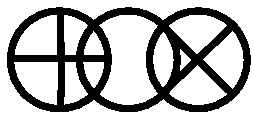
\includegraphics[width=20pt]{figures/logo1}
  }
\date{31st January 2019 - \textbf{AAAI19 \emph{Honolulu}}}
% \institute{Department of Computer Science, University of Bari ``Aldo Moro'', Bari, Italy
% \and 
% Department of Physics, University of Bari ``Aldo Moro'', Bari, Italy
% \and
% National Institute for Nuclear Physics (INFN), Bari Division, Bari, Italy
% }

% \institute{\textbf{Max-Planck-Institute}
%       \par \textbf{for Intelligent Systems}}
% \department{Probabilistic Learning}
\institutelogo{figures/mpi-minerva}
\institutesize{30pt}

% \secondinstitute{\textbf{TU Darmstadt}}
% \seconddepartment{Computer Science\\Department}
\secondinstitutelogo{figures/tu-darmstadt-athena.png}
\secondinstitutesize{25pt}

% \thirdinstitute{\textbf{University of} \\\textbf{Cambridge}}
% \thirddepartment{Engineering Department}
\thirdinstitutelogo{figures/cam-logo-big.png}
\thirdinstitutesize{25pt}


% \lablogo{\includegraphics[height=25pt]{figures/cam-logo-big-gray}}
% \otherlogo{\includegraphics[height=35pt]{figures/darms}}
% \otherlaboratory{TU Darmstadt}
% \othergroup{Computer Science Department}

\makeatletter
% \addtobeamertemplate{headline}{\vspace{-30pt}}{\hspace{10pt}}
% \defbeamertemplate*{frametitle}{custom-spinaceto}[1][]
% {
%   \vskip15pt%
%   \insertframetitle\par
%   \ifdefined\insertframesubtitle
%   \usebeamerfont{framesubtitle}\insertframesubtitle
%   \fi
% }
% \makeatother


{
  \setbeamertemplate{headline}{}
  \setbeamertemplate{footline}{}
  \begin{frame}
    \titlepage
  \end{frame}
}




\begin{frame}[t, htt=gold2]
  \frametitle{In a nutshell}
  \framesubtitle{or why should you care about SPNs}
  \small

  A short tutorial on\\[5pt]
  \hspace{105pt}\htt[tomato4]{\emph{\textbf{Sum-Product Networks}}
    (\textbf{SPNs})}~\emph{\parencite{Poon2011}}\\[5pt]

  an appealing deep and
          {\emph{\textbf{tractable density estimator}}} allowing {\emph{\textbf{exact inference}}}
          \\[20pt]

  Plus, SPNs can be \htt[bgrey2]{\emph{\textbf{interpreted}}} as {\emph{\textbf{hierarchical latent
      variable}}} (LV)
  probabilistic models,
  {\emph{\textbf{Multi-layer
        perceptrons}}}, and special kind of {\emph{\textbf{Arithmetic
  Circuits}}} and even \emph{\textbf{Bayesian Networks}}\\[20pt]
  
 Briefly reviewing representation capabilities,
 \htt[peas5]{\emph{\textbf{inference}}} and \htt[olive4]{\emph{\textbf{learning}}} schemes with
  SPNs\\[20pt]

  Ultimately touching some \htt[lacamgold5]{\emph{\textbf{applications}}}, extensions and research ideas\\[20pt]

  
\end{frame}


\begin{frame}[t]
  \frametitle{Notation}

  \begin{table}[t]
    \begin{tabular}{l r}
    $X, Y, Z, \dots$ & random variables (RVs) \\
    $\mathsf{val}(X)$ & support of RV $X$ \\
    $x\sim X$ & $x$ is drawn/distributed according to $X$ or
    $x\in\mathsf{val}(X)$\\
    $\mathbf{X} = (X_1, X_2, \dots, X_n)$ & ordered set of RVs \\
    $\mathbf{x}\sim \mathbf{X},\mathbf{x}= \langle x_1, x_2, \dots, x_n\rangle$ &
    multivariate sample from $\mathbf{X}$\\
    $\mathbf{x}_{|\mathbf{Y}}$ & restriction of sample $\mathbf{x}$ to
    RVs $\mathbf{Y}\subset\mathbf{X}$ \\
    $p_{\mathbf{X}}, p$ & PMF or PDF over RVs $\mathbf{X}$\\
    $p_{\mathbf{X}, \mathbf{Y}}(\mathbf{x}, \mathbf{y})$, $p(\mathbf{x}, \mathbf{y})$ & joint distribution over $\mathbf{X}\cup\mathbf{Y}$\\
    $p_{\mathbf{Y}| \mathbf{x}}(\mathbf{y}|\mathbf{x})$,
    $p(\mathbf{Y}|\mathbf{x})$ & conditional probability distribution\\
      \end{tabular}
    \end{table}
    \customcite{Poon2011}
    \footfullcitenomarkleft{Poon2011}
    \footnote{Poon is great}
\end{frame}


\begin{frame}[t]
  \frametitle{\htt[lacamdarklilac]{Density estimation}}

  Unsupervisedly learning an estimator for the joint probability distribution
    $p(\mathbf{X})$ from a set of i.i.d. samples $\mathcal{D}=\{\mathbf
    x^i\}_{i=1}^m$ over random variables (RVs) $\mathbf{X}=\{X_{1},\dots,X_{n}\}$\customcite{Poon2011}\\[17pt]
    
    Given such an estimator, one uses it to \textbf{\emph{answer
    probabilistic queries}} about configurations on $\mathbf{X}$,
i.e. to do \emph{\textbf{inference}}.\par
\begin{minipage}{1.0\linewidth}
     \vspace{-25pt}
          \raggedleft
          {$\color{violet}\boldsymbol\Rightarrow$
          {\footnotesize
            \emph{most ML task can be reframed as probabilistic inference!}\\
          }}
      
     
\end{minipage}\\[17pt]

    The \textbf{inherent trade-off} in density estimation: balancing
    \begin{itemize}
      \setlength\itemsep{0pt}
    \item the \htt[purple]{\textbf{\emph{representation
            expressiveness}}} of the model to learn
      \item the \htt[petroil2]{\textbf{\emph{cost of performing inference}}} on it
    \item and the \htt[gold2]{\textbf{\emph{cost of learning}}}
      such a model
      
    \end{itemize}

\end{frame}



\begin{frame}[t]
  \frametitle{\htt[lacamdarklilac]{\emph{(Different kinds of)} Inference}}
%   Different types of models make different operations tractable

% \vskip 10pt

% Operations that may be required to be efficient are
  \begin{minipage}[t]{0.9\linewidth}
    \begin{itemize}
      \setlength{\itemsep}{7pt}
    \item complete evidence ({\footnotesize$\mathsf{EVI}$})\hfill
      {\scriptsize$p(\mathbf{X} = \mathbf{x})$}
      % \hfill {\color{violet} $\rightarrow$ tractable for SPNs, BNs}
    \item 
      marginals ({\footnotesize$\mathsf{MAR}$})\hfill {\scriptsize$p(\mathbf{E=\mathbf{e}}),\quad \mathbf{E}\subset\mathbf{X}$}
      % \hfill {\color{violet} $\rightarrow$ tractable for SPNs, hard
      % in
      % BNs (even approximate)}
    \item
       conditionals ({\footnotesize$\mathsf{CON}$})\hfill {\scriptsize$p(\mathbf{Q}|\mathbf{E}),\quad \mathbf{Q},
      \mathbf{E}\subset\mathbf{X}, \mathbf{Q}\cap
      \mathbf{E}=\emptyset$}
      
    \item
       Most Probable Explanation ({\footnotesize$\mathsf{MPE}$})\hfill {\scriptsize$\arg\max_{\mathbf{q}\sim\mathbf{Q}}p(\mathbf{q}|\mathbf{E}),\quad
      \mathbf{Q}\cup \mathbf{E}=\mathbf{X}, \mathbf{Q}\cap
      \mathbf{E}=\emptyset$}
    \item  Maximum A
      Posteriori ({\footnotesize$\mathsf{MAP}$}) \hfill
      {\scriptsize$\arg\max_{\mathbf{q}\sim\mathbf{Q}}\sum_{\mathbf{h}\sim\mathbf{H}}p(\mathbf{q},\mathbf{h}|\mathbf{E})$}\par
      \hfill{\scriptsize$\mathbf{Q}\cup\mathbf{H}\cup \mathbf{E}=\mathbf{X},
      \mathbf{Q}\cap\mathbf{H}=\emptyset,\mathbf{Q}\cap
      \mathbf{E}=\emptyset, \mathbf{H}\cap \mathbf{E}=\emptyset$}
      % \hfill {\color{violet} $\rightarrow$ hard for both SPNs and
      % BNs}
    \item 
      partition function computation \hfill {\scriptsize$Z = \sum_{\mathbf{x}}\phi(\mathbf{x})$}
      % \hfill {\color{violet} $\rightarrow$ tractable for SPNs, hard
      % for MNs}
    \item sampling ({\footnotesize$\mathsf{SAM}$}): generate independent samples from $p$
    \end{itemize}
  \end{minipage}\par\bigskip
    We strive for \textbf{\emph{exact}} inference, computable in \emph{\textbf{tractable}} time,
    i.e. polynomial in $|\mathbf{X}|$
\end{frame}








\begin{frame}[t]
    \frametitle{\htt[tomato3]{SPNs: exact and tractable inferences}}
    \footnotesize
    \vspace{5pt}
    Let $\nodeset{S}^{\oplus}$ (resp. $\nodeset{S}^{\otimes}$) be the set of all sum
    (resp. product) nodes in an SPN $S$, then 
    \begin{itemize}
      \setlength{\itemsep}{0pt}  
\item    $S$ is \htt[tomato0]{\emph{\textbf{complete}}} iff $\forall n\in
  \nodeset{S}^{\oplus},\forall c_{1}, c_{2}\in \mathsf{ch}(n):
  \mathsf{sc}(c_{1})=\mathsf{sc}(c_{2})$
\item    $S$ is \htt[tomato0]{\emph{\textbf{decomposable}}} iff $\forall n\in
  \nodeset{S}^{\otimes},\forall c_{1}, c_{2}\in \mathsf{ch}(n)% , c_{1}\neq c_{2}
  :
  \mathsf{sc}(c_{1})\cap\mathsf{sc}(c_{2})=\emptyset$
\end{itemize}\par\bigskip

If $S$ is complete and decomposable,  it is
 \htt[tomato0]{\emph{\textbf{valid}}},
and it exactly
computes, in \textbf{time linear w.r.t. to its size}
$|S|$\customcite{Darwiche2009}\customcite{Poon2011}:
\begin{minipage}{1.0\linewidth}
  \vspace{2pt}
      \raggedleft
      $\color{violet}\boldsymbol\Rightarrow$
\emph{caveat:  $|S|$ shall be polynomial in $|\mathbf{X}|$\dots}
\end{minipage}\\[-10pt]
% \begin{minipage}{1.0\linewidth}
%       \vspace{-10pt}
%       \raggedleft
%       $\color{violet}\boldsymbol\Rightarrow$    
% % \hfill$\rightarrow$
% \emph{\textbf{evidence}, \textbf{marginals}, \textbf{Z}} in time
% linear to $|S|$
% \end{minipage}
\begin{itemize}
  \setlength{\itemsep}{0pt}  
\item  complete evidence $p(\mathbf{X}=\mathbf{x})$
\item marginals $\quad p(\mathbf{Q}=\mathbf{q})$, conditionals $\quad p(\mathbf{Q}=\mathbf{q}|\mathbf{e})$
\item partition function $\mathbf{Z}$
\end{itemize}
\par\bigskip

An SPN $S$ is 
\htt[tomato0]{\textbf{\emph{selective}}}~\customcite{Peharz2014b}, iff $\forall \mathbf{x}^{i}\sim\mathbf{X},\forall
n\in\nodeset{S}^{\oplus}\colon
|\{c \cbar c\in\mathsf{ch}(n):S_{c}(\mathbf{x}^{i})>0\}|
\leq 1$\par
% \hfill$\rightarrow$
\begin{minipage}{1.0\linewidth}
  \vspace{2pt}
      \raggedleft
      $\color{violet}\boldsymbol\Rightarrow$|S|
\emph{\textbf{MPE inference}, \textbf{assignments}} in time
linear to $|S|$
\end{minipage}\customcite{Choi2017}
\end{frame}



\begin{frame}[t]
\frametitle{\htt[bgrey1]{Trivia: Interpreting SPNs}}

An SPN encodes a \emph{\textbf{multi-linear function}} in a compact data structure~\customcite{Darwiche2009}
   \begin{minipage}{0.9\linewidth}
 %     \vspace{2pt}
      \raggedleft
      $\color{violet}\boldsymbol\Rightarrow$
      \scriptsize
     \emph{a giant (network) polynomial over $\mathbf{X}$!}
   \end{minipage}\par\bigskip


SPNs are \textbf{not PGMs}! They are \emph{\textbf{computational graphs}}
\begin{minipage}{0.9\linewidth}
 %     \vspace{2pt}
      \raggedleft
      % {\scriptsize
     % \emph{their DAG represents a computational graph not conditional
     %   independencies}}
   $\color{violet}\boldsymbol\Rightarrow$
      {\scriptsize
     \emph{equivalent to Arithmetic Circuits for finite discrete domains}}
\end{minipage}~\customcite{Rooshenas2014}\par\bigskip


SPNs are \htt[bgrey2]{\emph{\textbf{hierarchical LV probabilistic}}} models 
\begin{minipage}{0.9\linewidth}
 %     \vspace{2pt}
      \raggedleft
      $\color{violet}\boldsymbol\Rightarrow$
      {\scriptsize
     \emph{one can think of them as the {\textbf{deep version of mixture models}}}}\par
   % $\color{violet}\boldsymbol\Rightarrow$
   %    {\scriptsize
   %   \emph{ancestral sampling routines can be devised}}
\end{minipage}\par\bigskip

SPNs are peculiar \htt[bgrey4]{\emph{\textbf{feedforward neural networks}}} 
\begin{minipage}{0.9\linewidth}
 %     \vspace{2pt}
      \raggedleft
      $\color{violet}\boldsymbol\Rightarrow$
      \scriptsize
     \emph{reparameterizable as \textbf{sparse}, \textbf{constrained}, \textbf{fully-probabilistic} MLPs}
\end{minipage}~\customcite{Vergari2016a}\par\bigskip

\end{frame}

   
 
\begin{frame}[allowframebreaks]
  \frametitle{References}
  \setlength\bibitemsep{8pt}
  \printbibliography
\end{frame}

out
\end{document}

%%% Local Variables:
%%% mode: latex
%%% TeX-engine: xetex
%%% TeX-master: t
%%% End:
